\chapter{Présentation d'un jeu d'essai}\label{ch:jeu-essai}

Ce chapitre présente le fonctionnement de l'API Pipeline documentaire illustré par des captures d'écran. Nous suivons le comportement de l'API à travers les étapes suivantes :

\begin{enumerate}
    \item Nous envoyons une requête POST à l'API à l'aide de Postman pour importer un fichier des transactions de carburant, en l'occurrence, un fichier LCCC. Ensuite, Postman affiche la réponse réussie de l'API (code 201, identifiant et statut du téléchargement) (Figure~\ref{fig:postman}).
    \item Dans le terminal du conteneur Docker de l'application, où la file d'attente de Laravel a été préalablement démarrée à l'aide de la commande \Verb|php artisan queue:listen|, nous pouvons voir la liste des maillons au fur et à mesure que la file d'attente les exécute (Figure~\ref{fig:docker}).
    \item Simultanément, dans la base de données de l'application, nous constatons l'ajout d'un nouvel enregistrement dans la table des téléchargements (\Verb|uploads|). De plus, dans la table des maillons de téléchargement (\Verb|upload_steps|), plusieurs nouveaux enregistrements sont créés pour refléter chaque maillon du traitement du fichier (Figure~\ref{fig:uploads_upload_steps}).
    \item Dans la base de données \Verb|suivideflotte|, les données extraites du fichier sont ajoutées à la table \Verb|23-02_gaz_tid_transaction|, et un nouvel enregistrement est créé dans la table \Verb|gaz_tid_import_historique| pour consigner le succès de l'importation du fichier (Figure~\ref{fig:transaction_history}).
    \item Dans le dossier de stockage (\Verb|storage|) du projet \Verb|docker-pipeline|, le fichier d'origine ainsi que la charge utile sont enregistrés dans le répertoire \Verb|app/storage-directory|, tandis que les fichiers de sortie des différents maillons sont stockés dans le répertoire \Verb|app/work-directory| (Figure~\ref{fig:step-files}).
    \item Enfin, si nous retournons à Postman et tentons d'envoyer une charge utile qui ne contient pas toutes les données requises, l'API répondra avec une erreur 422 (Figure~\ref{fig:postman-error}).
\end{enumerate}

On voit que ce fonctionnement correspond aux exigences initiales formulées dans le cahier des charges du projet.

\begin{figure}[ht]
    \centering
    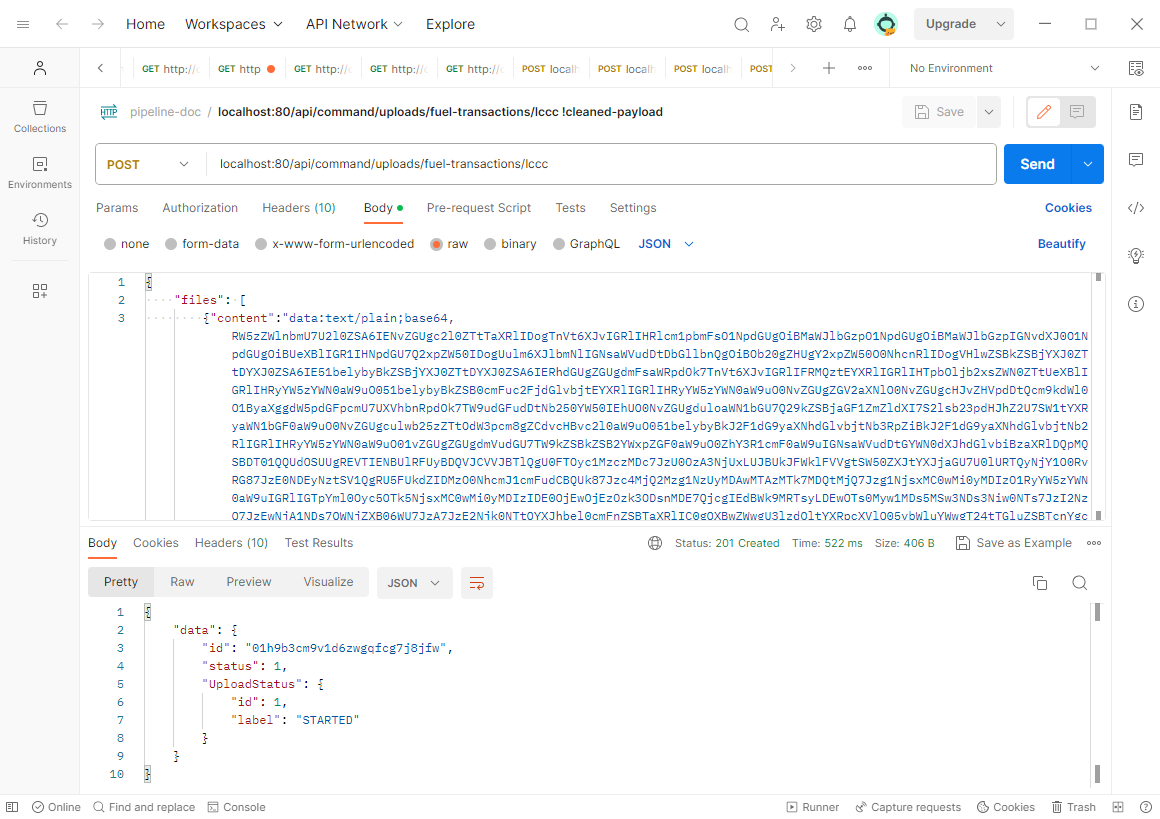
\includegraphics[width=\textwidth]{img/postman}
    \caption{Envoi d'un fichier LCCC à l'API Pipeline documentaire et réception d'une réponse réussie dans Postman.}
    \label{fig:postman}
\end{figure}

\begin{figure}[ht]
    \centering
    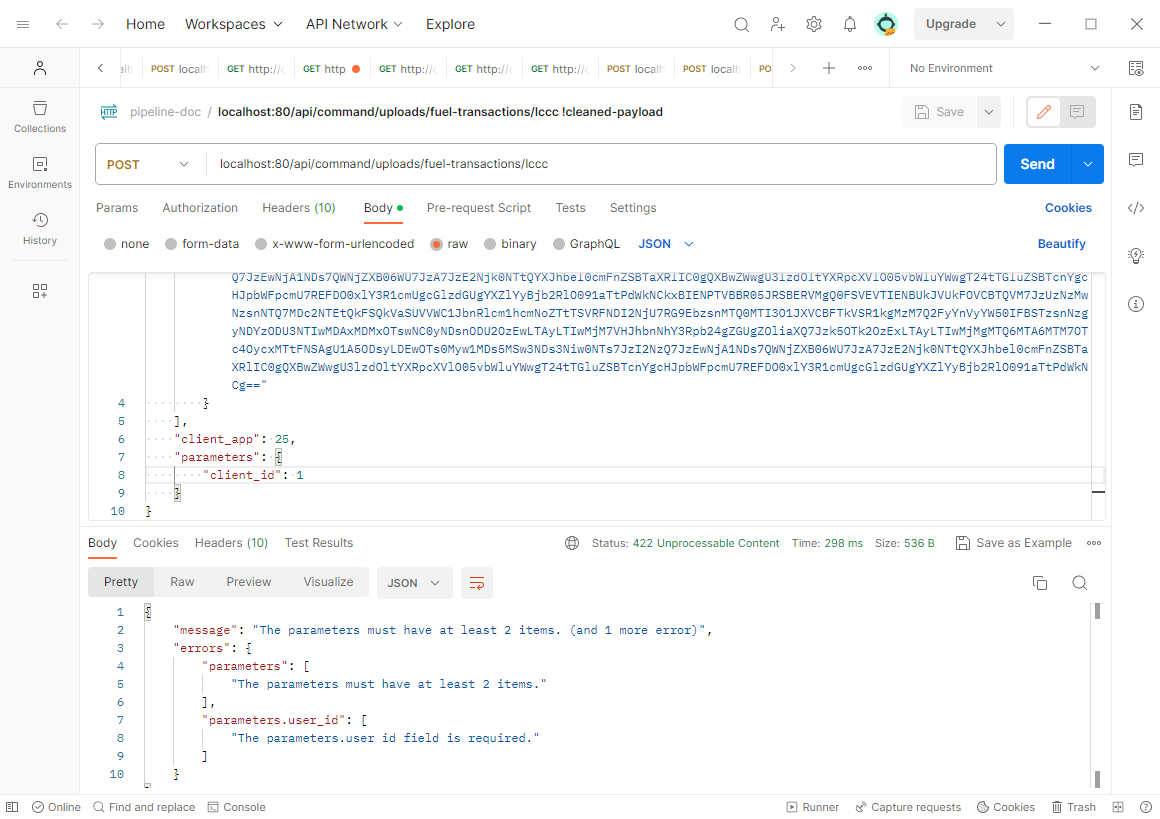
\includegraphics[width=\textwidth]{img/postman-error}
    \caption{L'API répond avec un code d'erreur (422) si nous envoyons un payload non complet (le \Verb{user_id} est manquant).}
    \label{fig:postman-error}
\end{figure}

\begin{figure}[ht]
    \centering
    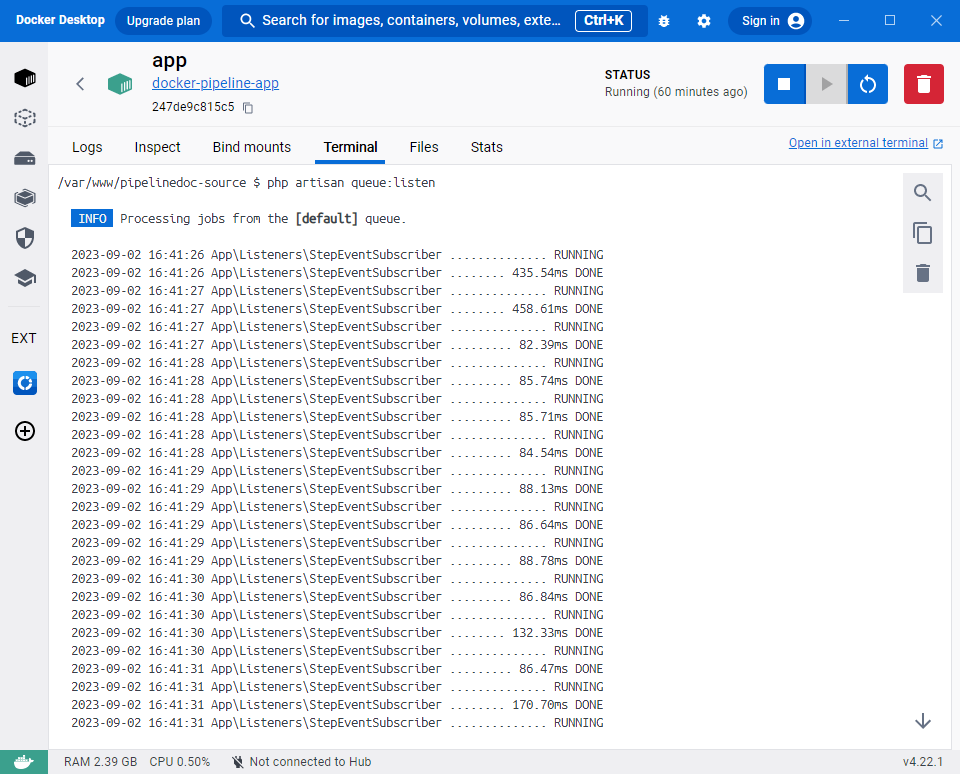
\includegraphics[width=\textwidth]{img/docker}
    \caption{Dans le terminal du conteneur Docker de l'application la liste des maillons est affichée au fur et à mesure que la file d'attente les exécute.}
    \label{fig:docker}
\end{figure}

\begin{figure}[ht]
    \centering
    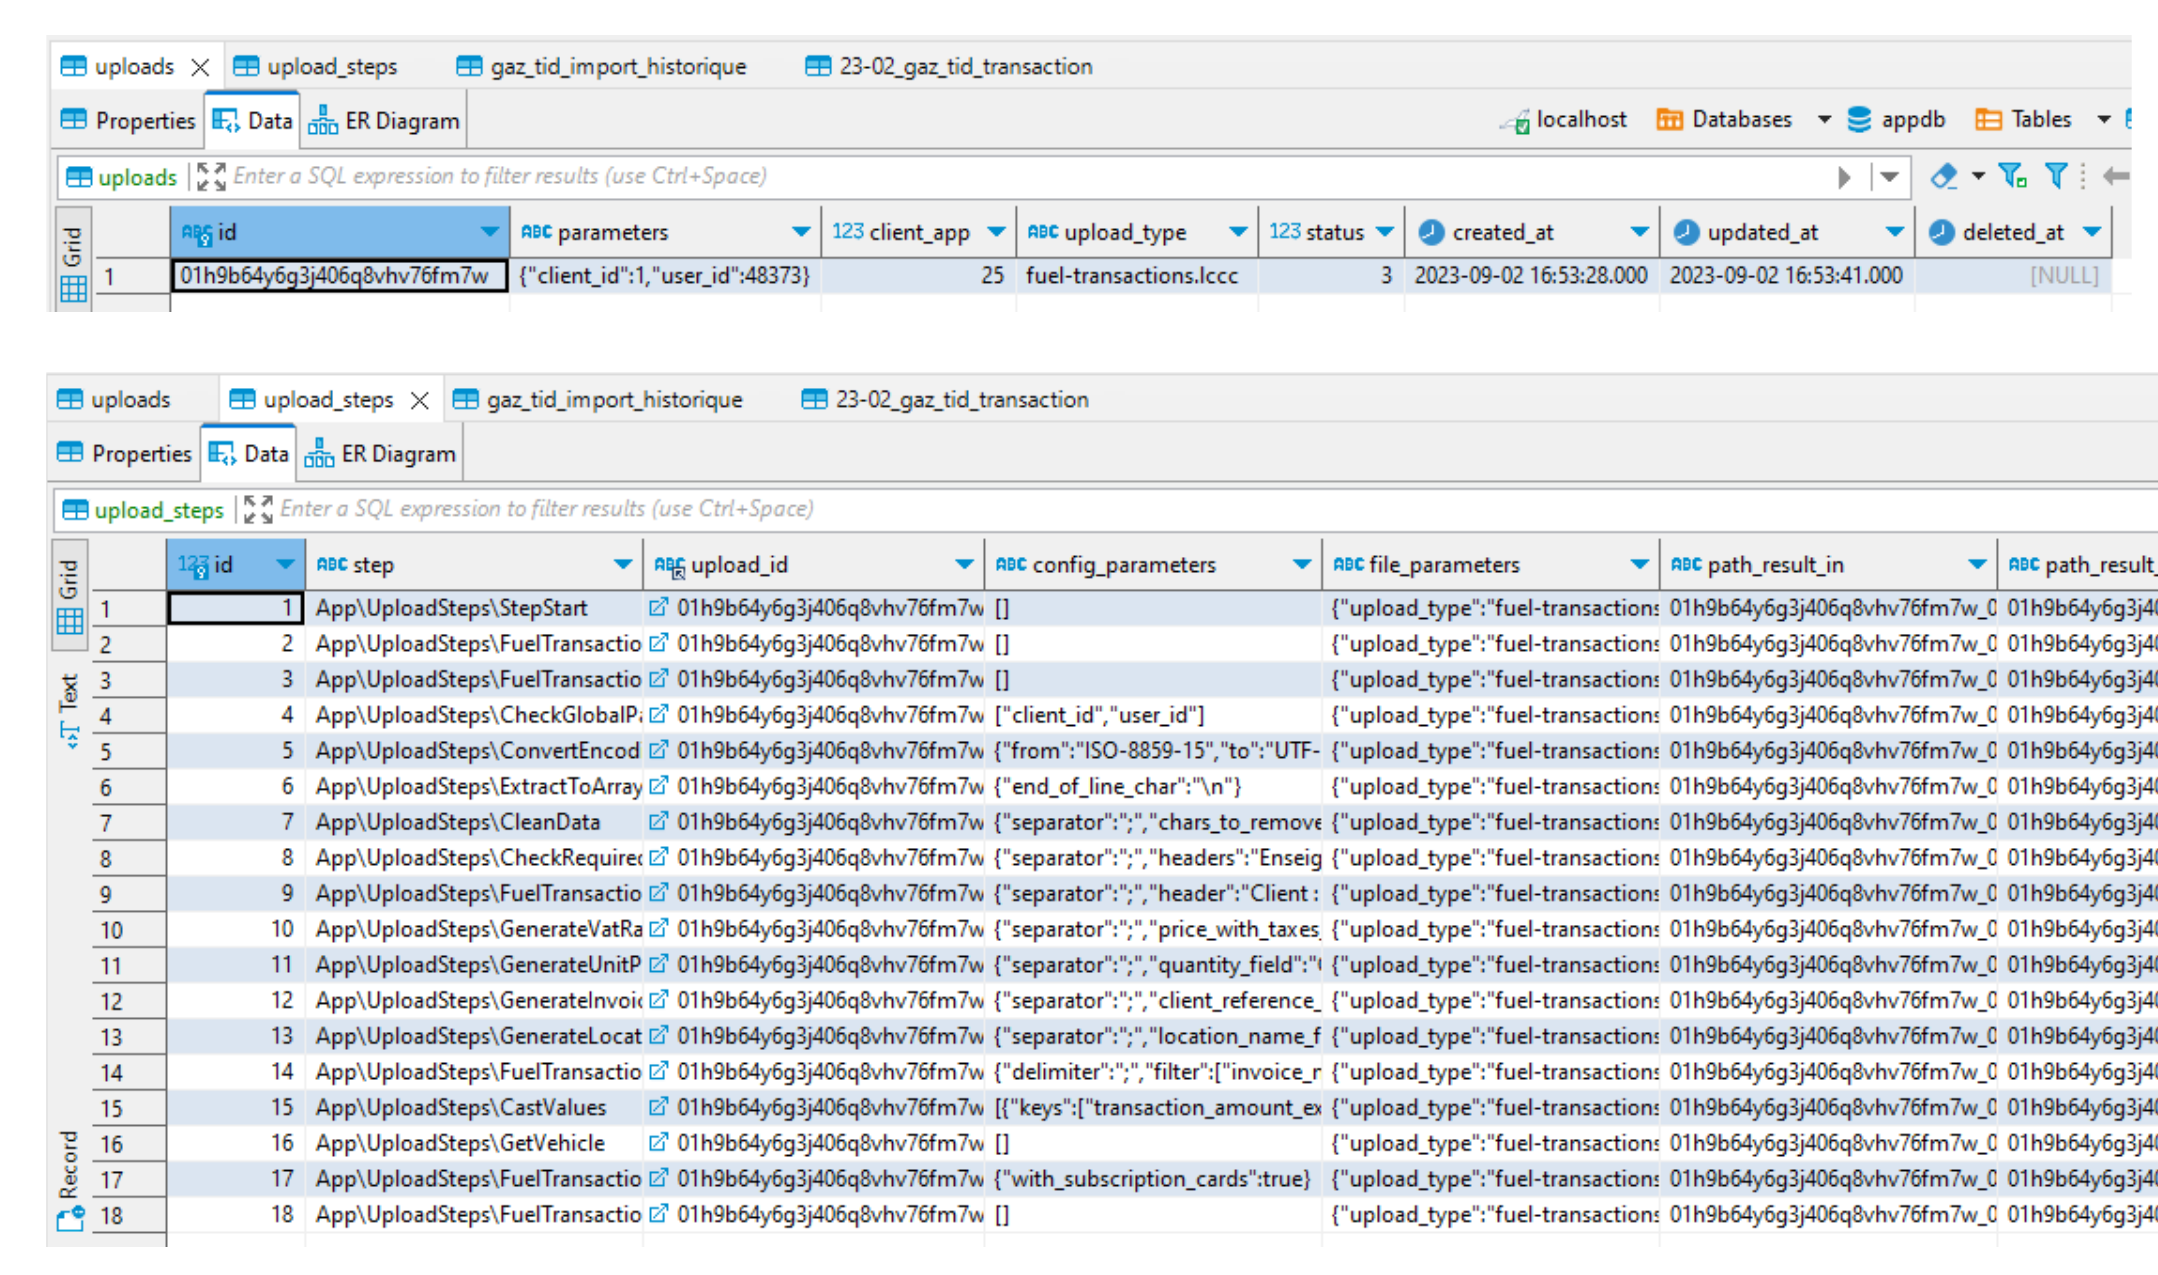
\includegraphics[width=\textwidth]{img/uploads_upload_steps}
    \caption{L'objet \Verb{Upload} et les objets \Verb{UploadStep} sont stockés dans les tables correspondantes de la base de données.}
    \label{fig:uploads_upload_steps}
\end{figure}

\begin{figure}[ht]
    \centering
    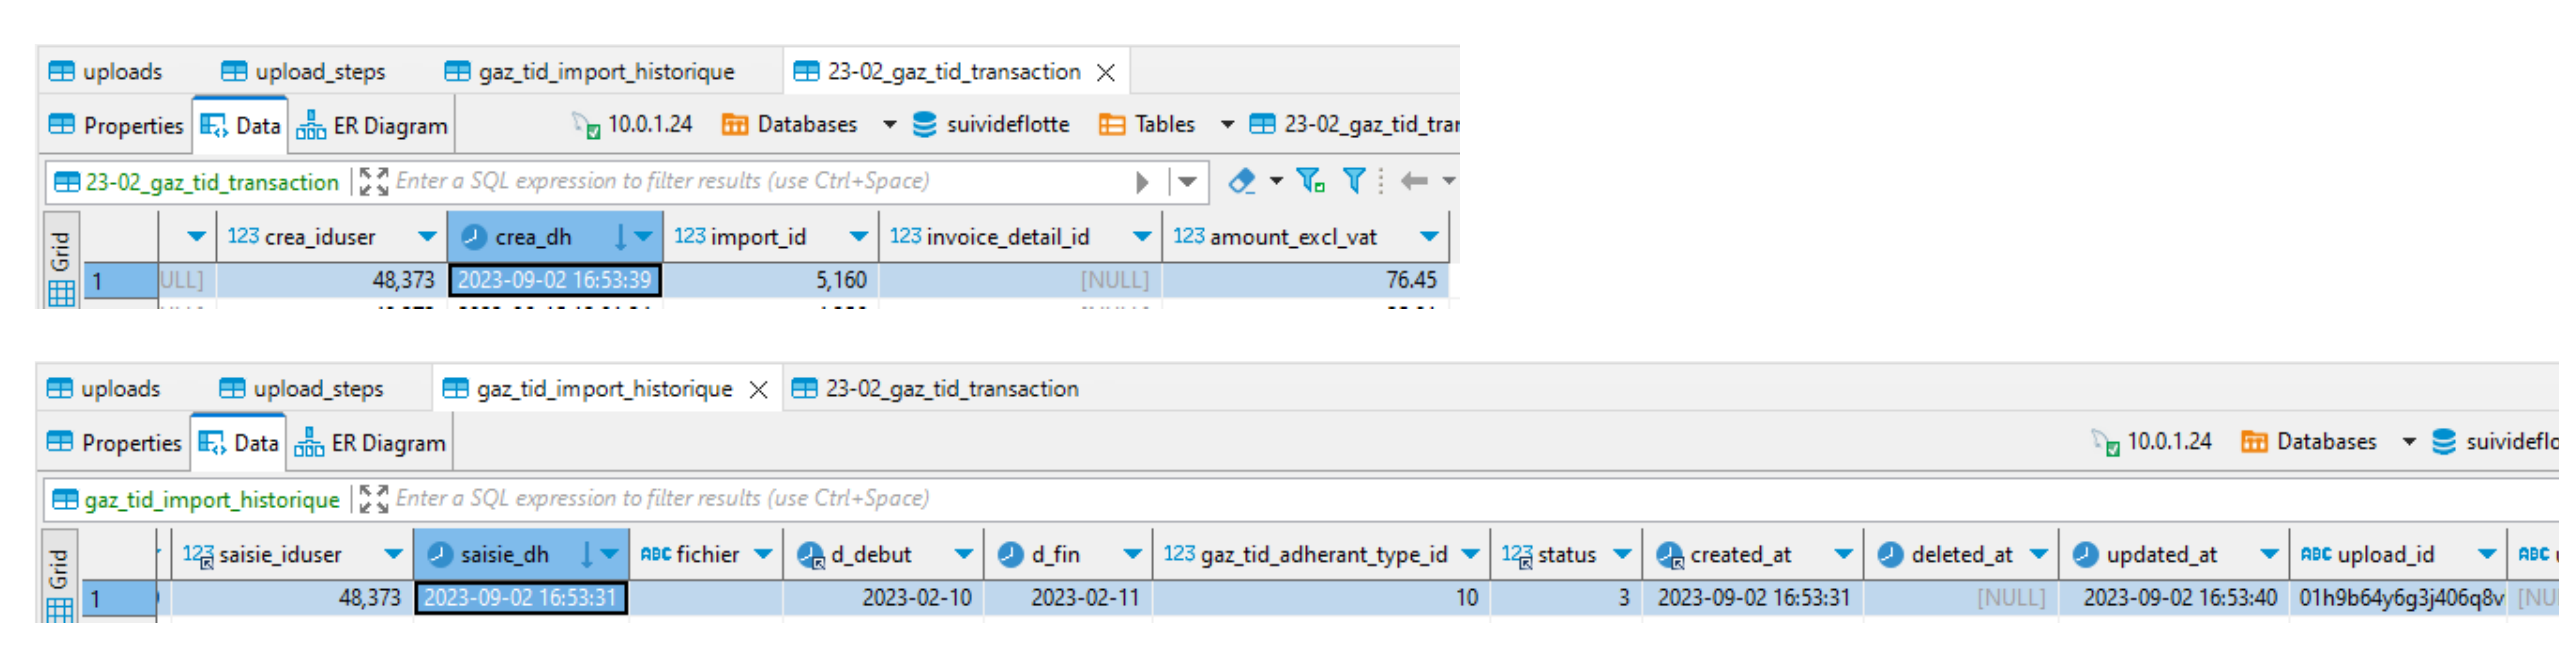
\includegraphics[width=\textwidth]{img/transaction_history}
    \caption{Dans la base de données \Verb{suivideflotte}, les données extraites du fichier sont ajoutées à la table \Verb{23-02_gaz_tid_transaction}, et un nouvel enregistrement est créé dans la table \Verb{gaz_tid_import_historique}.}
    \label{fig:transaction_history}
\end{figure}

\begin{figure}[ht]
    \centering
    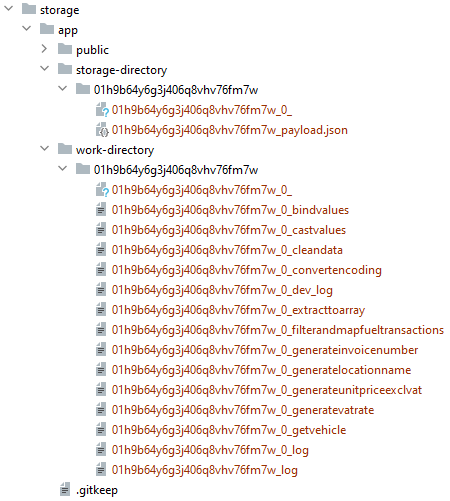
\includegraphics[width=0.9\textwidth]{img/step-files}
    \caption{Dans le dossier de stockage (\Verb{storage}) du projet \Verb{docker-pipeline}, le fichier d'origine ainsi que la charge utile sont enregistrés dans le répertoire \Verb{app/storage-directory}, tandis que les fichiers de sortie des différents maillons sont stockés dans le répertoire \Verb{app/work-directory}.}
    \label{fig:step-files}
\end{figure}